\section{Tests}
\label{sec:tests}

This chapter will present two conducted tests. It should
be noted here that, like described in the Introduction,
these are not very comprehensive tests. This chapter rather
visualizes the use of the PCF predicting on partitions of
otherwise unpredictable datasets.

The first test will visualize what the descision surface of
the PCF looks like, the second will show how the PCF
behaves with different amounts of Trees.

Both tests are performed on a randomly generated,
normalized, two dimensional and binary labeled dataset. The
dataset contains five thousand observations and was
designed to be unpredictable, when predicted as a whole.
The plane from which the observations are generated
contains five partitions in which the observations all have
the same label. Observations from those five partitions
make up twenty percent of all observations and are the only
ones which should be predicted, because all points not
inside those partitions are labeled randomly. The optimal
descision surface would be equal to the area of the five
partitions.

All observations are generated by a pseudo-random number
generator\cite[chapter 9.6]{python}, therefore, every point
on the plane has the same probability to be chosen as an
observation for the dataset.

It is common practise in machine learning to split a
dataset into a training and a test set in order to find
the best model.\footnote{For splitting scikit-learn's
  model\_selection.train\_test\_split was used during the
  tests.\cite{sklearn_api}}\cite[chapter 18]{ki}
This approach is also used for the PCF. The training set is
used as the parameters $X$ and $y$ of FIT (Algorithm~%
\ref{alg:pcf_fit}) while PREDICT (Algorithm~%
\ref{alg:pcf_pred}) is used on every observation of the
test set.

Two metrics are used to describe the behaviour of the PCF,
(\romannumeral 1) $predicted$ and (\romannumeral 2)
$accuracy$. Both metrics are derived from comparing the
label of an observation returned by PREDICT with its actual
label from the dataset.

$Predicted$ is the percentage of predicted observations,
while $accuracy$ is the percentage of correctly classified
observartions from the test set.

For both tests $\gamma$, $\tau_l$ and $\tau_h$ are the
same. $\gamma$ and $\tau_l$ are equal to the values used in
Figure~\ref{fig:fit_example} while $\tau_h = 32$. The
dataset was splitted into a training and a test set such
that ten percent of the observations were used as the test
set. The observations were chosen randomly.

The first test will show the descision surface of the PCF
with different $N$ and $\tau_{|X|}$. For the test three
different values, two, five and ten were used for both $N$
and $\tau_{|X|}$ to show how those two parameters change
the descision surface of the PCF. The test shows that for
$\tau_{|X|} = 2$ the PCF overfitted the data, which means
that $predicted$ exceeded twenty percent, the amount of
accurate observations while also failing to meet an
$accuracy$ equal to $\tau_l$. This results in the chaotic
descision surfaces shown in Figures~\ref{fig:x2_n2} -
\ref{fig:x2_n10}. On the other hand for $\tau{|X|} = 10$
the descision surface is very small which means the PCF's
$predicted$ is less than twenty percent (Figures~%
\ref{fig:x10_n2} - \ref{fig:x10_n10}).

The second test shows the influence the amount of Trees $N$
has on $predicted$ and $accuracy$. In this test
$\tau_{|X|}$ equals four.

Figure~\ref{fig:n} shows that, for this dataset with the
chosen thresholds, $N < 30$ has variations, both in
$predicted$ and $accuracy$. Is $30 \leq N \leq 100$
$accuracy$ is constant and equals $\tau_l$. $Predicted$ on
the other hand, still rises in this interval. Is
$N \geq 100$ $predicted$ is higher than $predicted$ with
$N = 100$ and constant, but $accuracy$ fails to meet
$\tau_l$, which means the PCF is overfitting.

Furthermore the second test relates $predicted$ and
$accuracy$ of the observations from the test set to the
values for the training set, showing that more training
observations are predictable than test observations
(cmp. Figure~\ref{fig:n}).


% TODO:
%       cite (chapter)

\def\setmeshr#1{
  \def\meshr{#1}
}
\def\meshr{1pt}

\pgfooclass{meshgrid visualizer}{
  % Stores the name of the visualizer. This is needed for
  % filtering and configuration
  \attribute name;

  % The constructor. Just setup the attribute.
  \method meshgrid visualizer(#1) { \pgfooset{name}{#1} }

  % Connect to visualize signal.
  \method default connects() {
    \pgfoothis.get handle(\me)
    \pgfkeysvalueof{/pgf/data visualization/obj}.connect(
      \me,visualize,visualize datapoint signal)
  }

  % This method is invoked for each data point. It checks
  % whether the data point belongs to the correct
  % visualizer and, if so, calls the macro \dovisualization
  % to do the actual visualization.
  \method visualize() {
    \pgfdvfilterpassedtrue
    \pgfdvnamedvisualizerfilter
    \ifpgfdvfilterpassed
      \dovisualization
    \fi
  }
}

\def\dovisualization{
  \pgfkeysvalueof{%
    /data point/\pgfoovalueof{name}/execute at begin%
  }

  \pgfpointdvdatapoint
  \pgfgetlastxy{\macrox}{\macroy}

  \pgfmathsetmacro\xlow {\macrox - \meshr}
  \pgfmathsetmacro\ylow {\macroy - \meshr}
  \pgfmathsetmacro\xhigh{\macrox + \meshr}
  \pgfmathsetmacro\yhigh{\macroy + \meshr}

  \pgfpathrectanglecorners{\pgfpoint{\xlow}{\ylow}}
                          {\pgfpoint{\xhigh}{\yhigh}}

  \pgfkeysvalueof{%
    /data point/\pgfoovalueof{name}/execute at end%
  }
}
\tikzdatavisualizationset{
  visualize as meshgrid/.style={
    new object={
      when=after survey,
      store=/tikz/data visualization/visualizers/#1,
      class=meshgrid visualizer,
      arg1=#1
    },
    new visualizer={#1}{%
      color=visualizer color,
      every path/.style={fill,draw,opacity=0.5},
    }{},
    /data point/set=#1
  },
  visualize as meshgrid/.default=meshgrid
}

\setmeshr{0.5pt}

\def\visualizeds#1{
  \begin{tikzpicture}
    \datavisualization [
      scientific axes=clean,
      visualize as meshgrid/.list={mesh0, mesh1},
      visualize as scatter/.list={data0, data1},
      x axis={label={$x_0$}},
      y axis={label={$x_1$}},
      mesh0={style={color=red!50}},
      mesh1={style={color=blue!50}},
      data0={style={mark=o, mark size=0.1pt,
        visualizer color=red}},
      data1={style={mark=o, mark size=0.1pt,
        visualizer color=blue}},
    ]
    data[headline={x, y}, read from file=#1.mesh_0.csv,
      set=mesh0]
    data[headline={x, y}, read from file=#1.mesh_1.csv,
      set=mesh1]
    data[headline={x, y}, read from file=#1.data_0.csv,
      set=data0]
    data[headline={x, y}, read from file=#1.data_1.csv,
      set=data1]
    ;
  \end{tikzpicture}
}

\def\dslegend{
  \begin{flushright}
    \begin{tikzpicture}
      \begin{scope}[label distance=2pt]
        \node[color=red, circle, draw,fill,
          label=right:label 0, inner sep=1.5pt] at (0,0)
            (l_zero) {};
        \node[color=blue, circle,draw,fill,
          label=right:label 1, below=0.2 of l_zero,
          inner sep=1.5pt] (l_one) {};
      \end{scope}

      \node[color=red!50,opacity=0.5,
        label=right:predicted 0, below=0.2 of l_one, fill,
        draw] (m_zero) {};
      \node[color=blue!50,opacity=0.5,below=0.2 of m_zero,
        label=right:predicted 1, fill, draw] (m_one) {};
    \end{tikzpicture}
  \end{flushright}
}

% descision surface figure {{{
\begin{figure*}
  \begin{comment}
  \begin{subfigure}[b]{0.3\textwidth}
    \centering
    \scalebox{0.7}{%
      \visualizeds{application/data/descision_surface/e2_ls2}}
    \caption{}
    \vspace{-0.5cm}
    \begin{align*}
      \tau_{|X|} = 2&, N = 2, \\
      predicted &= 0.37
, \\
      accuracy &= 0.670

    \end{align*}
    \label{fig:x2_n2}
  \end{subfigure}
  \begin{subfigure}[b]{0.3\textwidth}
    \centering
    \scalebox{0.7}{%
      \visualizeds{application/data/descision_surface/e5_ls2}}
    \caption{}
    \vspace{-0.5cm}
    \begin{align*}
      \tau_{|X|} = 2&, N = 5, \\
      predicted &= 0.308
, \\
      accuracy &= 0.721

    \end{align*}
    \label{fig:x2_n5}
  \end{subfigure}
  \begin{subfigure}[b]{0.3\textwidth}
    \centering
    \scalebox{0.7}{%
      \visualizeds{application/data/descision_surface/e10_ls2}}
    \caption{}
    \vspace{-0.5cm}
    \begin{align*}
      \tau_{|X|} = 2&, N = 10, \\
      predicted &= 0.298
, \\
      accuracy &= 0.792

    \end{align*}
    \label{fig:x2_n10}
  \end{subfigure}

  \begin{subfigure}[b]{0.3\textwidth}
    \centering
    \scalebox{0.7}{%
      \visualizeds{application/data/descision_surface/e2_ls5}}
    \caption{}
    \vspace{-0.5cm}
    \begin{align*}
      \tau_{|X|} = 5&, N = 2, \\
      predicted &= 0.144
, \\
      accuracy &= 0.903

    \end{align*}
  \end{subfigure}
  \begin{subfigure}[b]{0.3\textwidth}
    \centering
    \scalebox{0.7}{%
      \visualizeds{application/data/descision_surface/e5_ls5}}
    \caption{}
    \vspace{-0.5cm}
    \begin{align*}
      \tau_{|X|} = 5&, N = 5, \\
      predicted &= 0.106
, \\
      accuracy &= 0.962

    \end{align*}
  \end{subfigure}
  \begin{subfigure}[b]{0.3\textwidth}
    \centering
    \scalebox{0.7}{%
      \visualizeds{application/data/descision_surface/e10_ls5}}
    \caption{}
    \vspace{-0.5cm}
    \begin{align*}
      \tau_{|X|} = 5&, N = 10, \\
      predicted &= 0.138, \\
      accuracy &= 1

    \end{align*}
  \end{subfigure}

  \begin{subfigure}[b]{0.3\textwidth}
    \centering
    \scalebox{0.7}{%
      \visualizeds{application/data/descision_surface/e2_ls10}}
    \caption{}
    \vspace{-0.5cm}
    \begin{align*}
      \tau_{|X|} = 10&, N = 2, \\
      predicted &= 0.076
, \\
      accuracy &= 1

    \end{align*}
    \label{fig:x10_n2}
  \end{subfigure}
  \begin{subfigure}[b]{0.3\textwidth}
    \centering
    \scalebox{0.7}{%
      \visualizeds{application/data/descision_surface/e5_ls10}}
    \caption{}
    \vspace{-0.5cm}
    \begin{align*}
      \tau_{|X|} = 10&, N = 5, \\
      predicted &= 0.074
, \\
      accuracy &= 1

    \end{align*}
    \label{fig:x10_n5}
  \end{subfigure}
  \begin{subfigure}[b]{0.3\textwidth}
    \centering
    \scalebox{0.7}{%
      \visualizeds{application/data/descision_surface/e10_ls10}}
    \caption{}
    \vspace{-0.5cm}
    \begin{align*}
      \tau_{|X|} = 10&, N = 10, \\
      predicted &= 0.068
, \\
      accuracy &= 1

    \end{align*}
    \label{fig:x10_n10}
  \end{subfigure}
  \end{comment}

  \dslegend

  \caption{The descision surfaces of differently configured
    PCFs. The threshold $\tau_{|X|}$ and the amount of
    Trees $N$ of the PCF are different for each Figure,
    \ref{fig:x2_n2} - \ref{fig:x10_n10}.}
  \label{fig:descision_surface}
\end{figure*}
% }}}

\begin{figure*}
  \begin{comment}
  \begin{subfigure}[b]{0.3\textwidth}
    \centering
    \scalebox{0.7}{%
      \visualizeds{application/data/other_classif/svm}}
    \caption{Support Vector Machine.}
    \vspace{-0.5cm}
    \begin{align*}
      Accuracy = 0.554
    \end{align*}
  \end{subfigure}
  \begin{subfigure}[b]{0.3\textwidth}
    \centering
    \scalebox{0.7}{%
      \visualizeds{application/data/other_classif/rf}}
    \caption{Random Forest.}
    \vspace{-0.5cm}
    \begin{align*}
      Accuracy = 0.596
    \end{align*}
  \end{subfigure}
  \begin{subfigure}[b]{0.3\textwidth}
    \centering
    \scalebox{0.7}{%
      \visualizeds{application/data/other_classif/nn}}
    \caption{K Nearest Neighbor.}
    \vspace{-0.5cm}
    \begin{align*}
      Accuracy = 0.56
    \end{align*}
  \end{subfigure}
  \end{comment}

  \dslegend

  \caption{The descision surfaces of other classifiers than
    the PCF.}
  \label{fig:other_classif}
\end{figure*}


\begin{figure*}
  \begin{subfigure}[b]{0.5\textwidth}
    \begin{tikzpicture}
      \datavisualization [
        scientific axes=clean,
        x axis={label={$N$}},
        y axis={label={Predicted}},
        visualize as line/.list={fit, pred},
        fit={style={color=red}},
        pred={style={color=blue}},
      ]
      data[headline={x, y}, read from file=tests/data/fit_known_4.csv,
        set=fit]
      data[headline={x, y}, read from file=tests/data/pred_known_4.csv,
        set=pred]
      ;
    \end{tikzpicture}
  \end{subfigure}
  \begin{subfigure}[b]{0.5\textwidth}
    \begin{tikzpicture}
      \datavisualization [
        scientific axes=clean,
        x axis={label={$N$}},
        y axis={label={Accuracy}},
        visualize as line/.list={fit, pred},
        fit={style={color=red}},
        pred={style={color=blue}},
      ]
      data[headline={x, y}, read from file=tests/data/fit_acc_4.csv,
        set=fit]
      data[headline={x, y}, read from file=tests/data/pred_acc_4.csv,
        set=pred]
      ;
    \end{tikzpicture}
  \end{subfigure}
  \begin{flushright}
    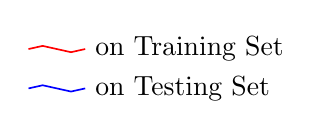
\begin{tikzpicture}
      \draw[red,semithick] (0,.5) -- (.18,.54) --
        (.54,.46) -- (.72,.5) node[right,black]
        {on Training Set};
      \draw[blue,semithick] (0,0) -- (.18,.04) --
        (.54,-.04) -- (.72,0) node[right,black]
        {on Testing Set};
    \end{tikzpicture}
  \end{flushright}
\end{figure*}


